\section{Visualization}
While users are searching their data, it is important to get statistically feedback
for their searches. Also, it is important to be able to at least do basic manipulation
on data and see what it means.

Vizualizations (Viz for short) do this. They allow users to see unique data, and graph 
values in comparison with other values. The Hatch Documents interface allow users to do 
things like catagorize data, and Viz graphs the results.

\begin{figure}[h]
	\begin{center}
	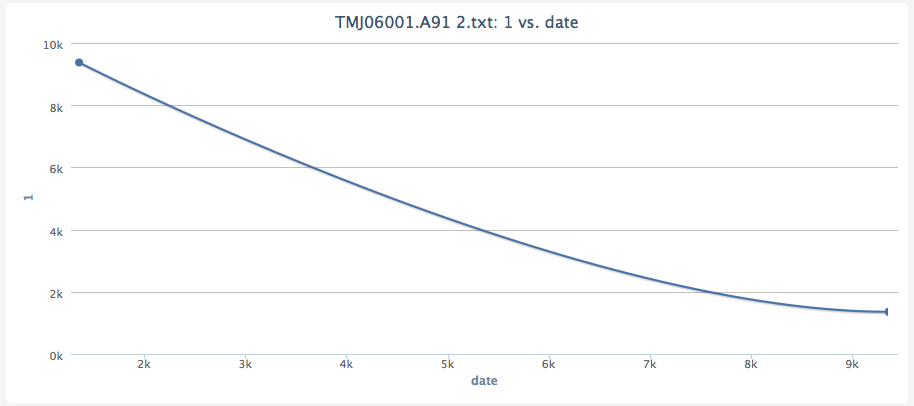
\includegraphics[width=120mm]{images/viz_ex1}
	\caption{A vizualization example.} 
	\label{viz_ex1}
	\end{center}
\end{figure}

Viz uses HighCharts, a JavaScript library. It allows Hatch to incrementally stream
new graph data to the client, instead of resending all the graph data. This is useful
when users are working on low bandwidth connections, or with large datasets. 

Viz also checks incrementally for new data. When Viz graphs data, it points towards the 
data in the document that needs visualization. If the data in the document changes,
Viz refreshes and graphs the new data.

This opens up the possibility of Feeds. Feeds are scheduled events in Hatch that pull
JSON data from somewhere on the web. They push the data in to the document they point
to, and Viz charts will detect an change in the document. 
The result is Live Charts, and documents that sync with data on the web when new data is 
available. Instead of doing a bulky request for data all at once, data can be taken
in smaller requests, and Viz can give users live feedback on their feeds.
